\documentclass[a4paper]{report}
% Some basic packages
\usepackage[utf8]{inputenc}
\usepackage[T1]{fontenc}
\usepackage{textcomp}
\usepackage[english]{babel}
\usepackage{url}
\usepackage{graphicx}
\usepackage{float}
\usepackage{booktabs}
\usepackage{enumitem}

\pdfminorversion=7

% Don't indent paragraphs, leave some space between them
\usepackage{parskip}

% Hide page number when page is empty
\usepackage{emptypage}
\usepackage{subcaption}
\usepackage{multicol}
\usepackage{xcolor}

% Other font I sometimes use.
% \usepackage{cmbright}

% Math stuff
\usepackage{amsmath, amsfonts, mathtools, amsthm, amssymb}
% Fancy script capitals
\usepackage{mathrsfs}
\usepackage{cancel}
% Bold math
\usepackage{bm}
% Some shortcuts
\newcommand\N{\ensuremath{\mathbb{N}}}
\newcommand\R{\ensuremath{\mathbb{R}}}
\newcommand\Z{\ensuremath{\mathbb{Z}}}
\renewcommand\O{\ensuremath{\emptyset}}
\newcommand\Q{\ensuremath{\mathbb{Q}}}
\newcommand\C{\ensuremath{\mathbb{C}}}
\renewcommand\L{\ensuremath{\mathcal{L}}}

% Package for Petri Net drawing
\usepackage[version=0.96]{pgf}
\usepackage{tikz}
\usetikzlibrary{arrows,shapes,automata,petri}
\usepackage{tikzit}
\input{petri_nets_style.tikzstyles}

% Easily typeset systems of equations (French package)
\usepackage{systeme}

% Put x \to \infty below \lim
\let\svlim\lim\def\lim{\svlim\limits}

%Make implies and impliedby shorter
\let\implies\Rightarrow
\let\impliedby\Leftarrow
\let\iff\Leftrightarrow
\let\epsilon\varepsilon

% Add \contra symbol to denote contradiction
\usepackage{stmaryrd} % for \lightning
\newcommand\contra{\scalebox{1.5}{$\lightning$}}

% \let\phi\varphi

% Command for short corrections
% Usage: 1+1=\correct{3}{2}

\definecolor{correct}{HTML}{009900}
\newcommand\correct[2]{\ensuremath{\:}{\color{red}{#1}}\ensuremath{\to }{\color{correct}{#2}}\ensuremath{\:}}
\newcommand\green[1]{{\color{correct}{#1}}}

% horizontal rule
\newcommand\hr{
    \noindent\rule[0.5ex]{\linewidth}{0.5pt}
}

% hide parts
\newcommand\hide[1]{}

% si unitx
\usepackage{siunitx}
\sisetup{locale = FR}

% Environments
\makeatother
% For box around Definition, Theorem, \ldots
\usepackage{mdframed}
\mdfsetup{skipabove=1em,skipbelow=0em}
\theoremstyle{definition}
\newmdtheoremenv[nobreak=true]{definitie}{Definitie}
\newmdtheoremenv[nobreak=true]{eigenschap}{Eigenschap}
\newmdtheoremenv[nobreak=true]{gevolg}{Gevolg}
\newmdtheoremenv[nobreak=true]{lemma}{Lemma}
\newmdtheoremenv[nobreak=true]{propositie}{Propositie}
\newmdtheoremenv[nobreak=true]{stelling}{Stelling}
\newmdtheoremenv[nobreak=true]{wet}{Wet}
\newmdtheoremenv[nobreak=true]{postulaat}{Postulaat}
\newmdtheoremenv{conclusie}{Conclusie}
\newmdtheoremenv{toemaatje}{Toemaatje}
\newmdtheoremenv{vermoeden}{Vermoeden}
\newtheorem*{herhaling}{Herhaling}
\newtheorem*{intermezzo}{Intermezzo}
\newtheorem*{notatie}{Notatie}
\newtheorem*{observatie}{Observatie}
\newtheorem*{exe}{Exercise}
\newtheorem*{opmerking}{Opmerking}
\newtheorem*{praktisch}{Praktisch}
\newtheorem*{probleem}{Probleem}
\newtheorem*{terminologie}{Terminologie}
\newtheorem*{toepassing}{Toepassing}
\newtheorem*{uovt}{UOVT}
\newtheorem*{vb}{Voorbeeld}
\newtheorem*{vraag}{Vraag}

\newmdtheoremenv[nobreak=true]{definition}{Definition}
\newtheorem*{eg}{Example}
\newtheorem*{notation}{Notation}
\newtheorem*{previouslyseen}{As previously seen}
\newtheorem*{remark}{Remark}
\newtheorem*{note}{Note}
\newtheorem*{problem}{Problem}
\newtheorem*{observe}{Observe}
\newtheorem*{property}{Property}
\newtheorem*{intuition}{Intuition}
\newmdtheoremenv[nobreak=true]{prop}{Proposition}
\newmdtheoremenv[nobreak=true]{theorem}{Theorem}
\newmdtheoremenv[nobreak=true]{corollary}{Corollary}

% End example and intermezzo environments with a small diamond (just like proof
% environments end with a small square)
\usepackage{etoolbox}
\AtEndEnvironment{vb}{\null\hfill$\diamond$}%
\AtEndEnvironment{intermezzo}{\null\hfill$\diamond$}%
% \AtEndEnvironment{opmerking}{\null\hfill$\diamond$}%

% Fix some spacing
% http://tex.stackexchange.com/questions/22119/how-can-i-change-the-spacing-before-theorems-with-amsthm
\makeatletter
\def\thm@space@setup{%
  \thm@preskip=\parskip \thm@postskip=0pt
}


% Exercise 
% Usage:
% \exercise{5}
% \subexercise{1}
% \subexercise{2}
% \subexercise{3}
% gives
% Exercise 5
%   Exercise 5.1
%   Exercise 5.2
%   Exercise 5.3
\newcommand{\exercise}[1]{%
    \def\@exercise{#1}%
    \subsection*{Exercise #1}
}

\newcommand{\subexercise}[1]{%
    \subsubsection*{Exercise \@exercise.#1}
}


% \lecture starts a new lecture (les in dutch)
%
% Usage:
% \lecture{1}{di 12 feb 2019 16:00}{Inleiding}
%
% This adds a section heading with the number / title of the lecture and a
% margin paragraph with the date.

% I use \dateparts here to hide the year (2019). This way, I can easily parse
% the date of each lecture unambiguously while still having a human-friendly
% short format printed to the pdf.

\usepackage{xifthen}
\def\testdateparts#1{\dateparts#1\relax}
\def\dateparts#1 #2 #3 #4 #5\relax{
    \marginpar{\small\textsf{\mbox{#1 #2 #3 #5}}}
}

\def\@lecture{}%
\newcommand{\lecture}[3]{
    \ifthenelse{\isempty{#3}}{%
        \def\@lecture{Lecture #1}%
    }{%
        \def\@lecture{Lecture #1: #3}%
    }%
    \subsection*{\@lecture}
    \marginpar{\small\textsf{\mbox{#2}}}
}



% These are the fancy headers
\usepackage{fancyhdr}
\pagestyle{fancy}

% LE: left even
% RO: right odd
% CE, CO: center even, center odd
% My name for when I print my lecture notes to use for an open book exam.
% \fancyhead[LE,RO]{Gilles Castel}

\fancyhead[RO,LE]{\@lecture} % Right odd,  Left even
\fancyhead[RE,LO]{}          % Right even, Left odd

\fancyfoot[RO,LE]{\thepage}  % Right odd,  Left even
\fancyfoot[RE,LO]{}          % Right even, Left odd
\fancyfoot[C]{\leftmark}     % Center

\makeatother




% Todonotes and inline notes in fancy boxes
\usepackage{todonotes}
\usepackage{tcolorbox}

% Make boxes breakable
\tcbuselibrary{breakable}

% Verbetering is correction in Dutch
% Usage: 
% \begin{verbetering}
%     Lorem ipsum dolor sit amet, consetetur sadipscing elitr, sed diam nonumy eirmod
%     tempor invidunt ut labore et dolore magna aliquyam erat, sed diam voluptua. At
%     vero eos et accusam et justo duo dolores et ea rebum. Stet clita kasd gubergren,
%     no sea takimata sanctus est Lorem ipsum dolor sit amet.
% \end{verbetering}
\newenvironment{verbetering}{\begin{tcolorbox}[
    arc=0mm,
    colback=white,
    colframe=green!60!black,
    title=Opmerking,
    fonttitle=\sffamily,
    breakable
]}{\end{tcolorbox}}

% Noot is note in Dutch. Same as 'verbetering' but color of box is different
\newenvironment{noot}[1]{\begin{tcolorbox}[
    arc=0mm,
    colback=white,
    colframe=white!60!black,
    title=#1,
    fonttitle=\sffamily,
    breakable
]}{\end{tcolorbox}}




% Figure support as explained in my blog post.
\usepackage{import}
\usepackage{xifthen}
\usepackage{pdfpages}
\usepackage{transparent}
\newcommand{\incfig}[1]{%
    \def\svgwidth{\columnwidth}
    \import{./figures/}{#1.pdf_tex}
}

% Fix some stuff
% %http://tex.stackexchange.com/questions/76273/multiple-pdfs-with-page-group-included-in-a-single-page-warning
\pdfsuppresswarningpagegroup=1


% My name
\author{Bruno M. Pacheco}

 
\begin{document}
 
\exercise{E1}

\subsubsection*{a)}

O sistema sem saturação possuí polinômio característico \[
    P(s) = s^{3}+6s^2 +5s+K
\], portanto, analisa-se sua estabilidade através do critério da matriz de Routh-Hurwitz para polinômios de grande ordem. A matriz

\begin{center}
\begin{tabular}{c c c}
    1 & 5 \\
    6 & $K$ \\
    $\frac{30-K}{6}$ & 0 \\
    $K$ & 0
\end{tabular}
\end{center}

nos indica que, para que o sistema ser estável, precisamos que
\begin{align*}
    \frac{30-K}{6} &> 0 \implies K<30 \\
	         K &> 0 \\
.\end{align*}

\subsubsection*{b)}

Para analisar o sistema com a saturação do tipo relê, aproximou-se o componente por um ganho equivalente. Utilizando uma aproximação de primeira ordem para a saturação, podemos substituir o componente por um ganho $N$ que depende da amplitude $A$ do sinal de entrada da saturação, ou seja,\[
    N(A) = \frac{4M}{\pi A} = \frac{4}{\pi A}
\].

Assim, podemos analisar a estabilidade através do polinômio característico do sistema em malha fechada considerando a aproximação da saturação de tipo relê \[
    P(s) = s^{3}+6s^2 +5s+KN(A)
\]. Utilizando novamente a matriz de Ruth-Hurwitz, pode-se atualizar os critérios de estabilidade utilizando o ganho $K' = KN(A)$ do sistema com saturação
\begin{align*}
    K' < 30 \implies \frac{K}{A} < \frac{30\pi}{4}\\
    K' > 0  \implies K > 0\\
.\end{align*}
Assim, validamos a ideia de que o ciclo limite se dá nas margens dos critérios de estabilidade, quando o sistema se torna oscilatório por causa dos polos puramente imaginários, através da trajetória das raízes, que pode ser vista na figura \ref{fig:figures-lab4_1_rlocus-png}.

\begin{figure}[H]
    \centering
    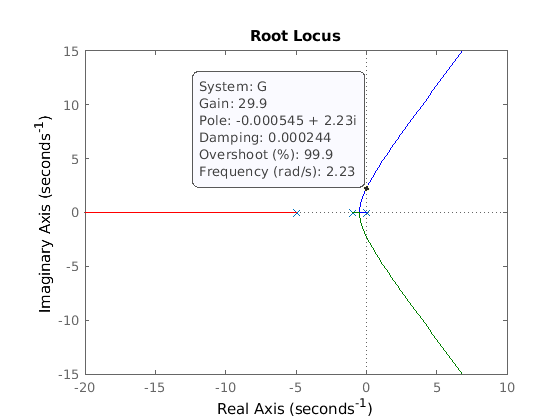
\includegraphics[width=0.6\textwidth]{figures/lab4_1_rlocus.png}
    \caption{Lugar das raízes do sistema.}
    \label{fig:figures-lab4_1_rlocus-png}
\end{figure}

Assim, vê-se que, de fato, o ciclo limite existirá para o caso $K' = 30$. Como tem-se já um valor pré-estabelecido para o ganho, tem-se que \[
    A > \frac{4K}{30\pi} \implies A > \frac{8}{3\pi}
\], em especial, no caso $A=\frac{8}{3\pi}$ tem-se o ciclo limite. Como $A$ é a amplitude na entrada da saturação, sabemos que o sinal após o primeiro integrador oscilará com uma amplitude de, aproximadamente, $0,85$ do ponto de referência, que, no caso, é $0$.

Para determinar a amplitude do ciclo limite, utilizou-se o diagrama de Nyquist da função de transferência com o ganho calculado para o ciclo limite, ou seja, espera-se que a trajetória cruze o ponto -1 do plano, indicando a presença de um ciclo limite. Assim, pode-se estimar a frequência do ciclo limite pela frequência da trajetória para o ponto $-1 + j0$, ou seja, o ponto limite de instabilidade. O diagrama de Nyquist pode ser observado na figura \ref{fig:figures-lab4_1_nyquist-png}. Estimou-se, então, a frequência do ciclo limite em $2,25$ rad/s.

\begin{figure}[H]
    \centering
    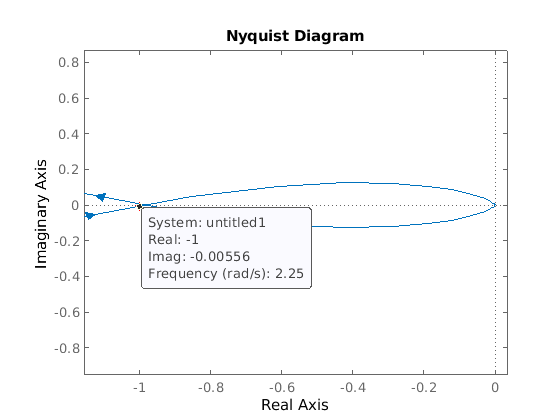
\includegraphics[width=0.8\textwidth]{figures/lab4_1_nyquist.png}
    \caption{Diagrama de Nyquist da função do sistema com ganho $K=20$ e o ganho equivalente da saturação que leva o sistema ao ciclo limite.}
    \label{fig:figures-lab4_1_nyquist-png}
\end{figure}

Simulou-se o sistema utilizando um modelo por variáveis de estado, à partir da equação, ignorando a saturação, do sistema no domínio do tempo \[
\ddot{y}(t) + 6\dot{y}(t) + 5y(t) = x_3(t)
\], onde $x_3(t)$ é a entrada da saturação. As variáveis escolhidas são \[
\begin{cases}
    x_1 = y(t) \\
    x_2 = \dot{y}(t) \\
    x_3 = \ddot{y}(t)
\end{cases}
\], o que resulta em um sistema em malha fechada \[
\begin{cases}
    \dot{x}_1(t) = x_2 \\
    \dot{x}_2(t) = -5x_1 -6x_2 + \phi(x_3) \\
    \dot{x}_3(t) = K(y_r(t) - y(t)) = K(y_r(t) - x_1(t))
\end{cases}
\], onde $\phi(.)$ é a função da saturação relé. A realização pode ser vista na figura \ref{fig:figures-lab4_1_modelo_simulink-png}.

\begin{figure}[H]
    \centering
    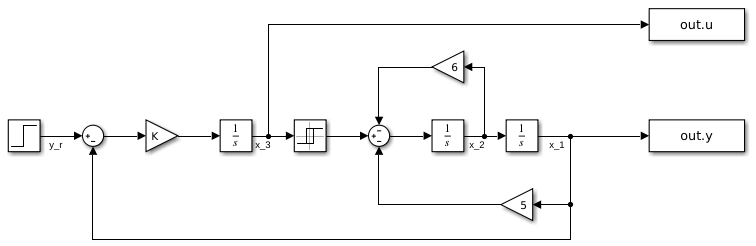
\includegraphics[width=0.8\textwidth]{figures/lab4_1_modelo_simulink.png}
    \caption{Modelo do sistema no software \emph{Simulink}.}
    \label{fig:figures-lab4_1_modelo_simulink-png}
\end{figure}

Os resultados da simulação com $y_r(t)=0$ podem ser observados nas figuras \ref{fig:figures-lab4_1_resposta_simulink} e \ref{fig:figures-lab4_1_b_states-png}.

\begin{figure}[H]
    \centering
    \begin{subfigure}{0.45\textwidth}
	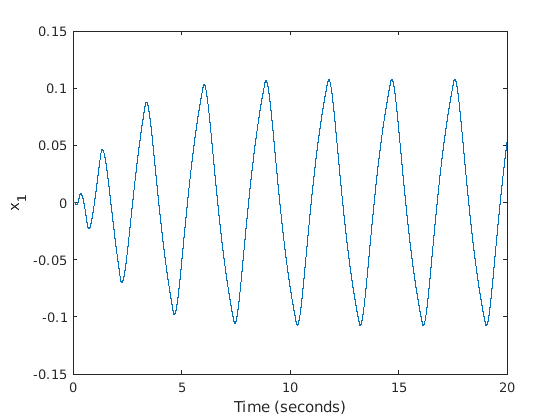
\includegraphics[width=\textwidth]{figures/lab4_1_y.png}
	\caption{Saída do sistema ($x_1$).}
    \end{subfigure}
    \begin{subfigure}{0.45\textwidth}
	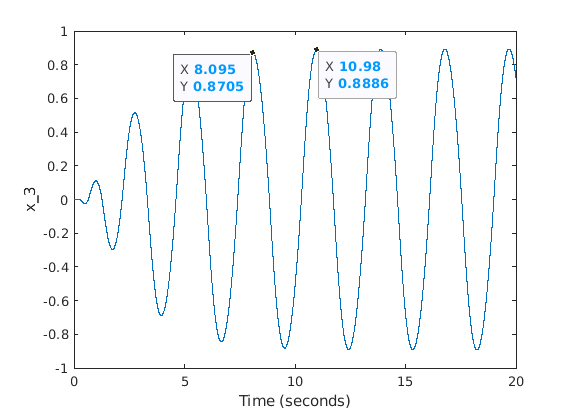
\includegraphics[width=\textwidth]{figures/lab4_1_x_3.png}
	\caption{Sinal de entrada da saturação do sistema ($x_3$).}
    \end{subfigure}
    \caption{Resposta do sistema à referência nula.}
    \label{fig:figures-lab4_1_resposta_simulink}
\end{figure}

\begin{figure}[H]
    \centering
    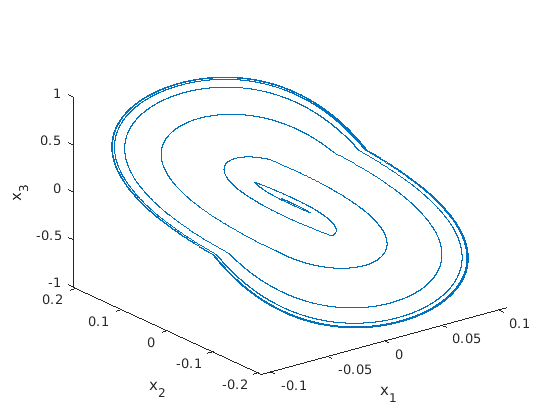
\includegraphics[width=0.6\textwidth]{figures/lab4_1_b_states.png}
    \caption{Espaço de estados do sistema com saturação do tipo relé.}
    \label{fig:figures-lab4_1_b_states-png}
\end{figure}

Observa-se a amplitude do sinal na entrada da saturação bastante próxima à estimada e um período também aproximadamente equivalente à frequência estimada. Supõe-se que os erros são decorrentes da aproximação feita do comportamento do componente de saturação.

\subsubsection*{c)}

À partir do sistema proposto, podemos calcular os equilíbrios através da derivada dos estados. Assim,
\begin{align*}
    &\dot{x}_1(t) = 0 \implies \overline{x}_2 = 0 \\
    &\dot{x}_2(t) = 0 \implies \phi \left( \overline{x}_3 \right) = 5\overline{x}_1 \\
    &\dot{x}_3(t) = 0 \implies \overline{x}_1 = y_r \\
,\end{align*}
ou seja, $y_r = \frac{1}{5}\phi \left( \overline{x}_3 \right) $. Como sabemos que $\phi:\R\to \left\{ -M, M \right\} $, então o equilíbrio não existe para $y_r \in (-M,M)$ e o sistema atinge um ciclo limite estável. O equilíbrio só é atingido quando $y_r(t) \in \left\{  \frac{-M}{5}, \frac{M}{5} \right\}$. Nota-se que a única condição sobre $\overline{x}_3$ é que ele concorde em sinal com a referência, tendo valor final determinado pelo tempo de acomodação do sistema e seu valor inicial. Sabemos que $\exists \lim_{t \to \infty} x_3(t)$, \emph{i.e.}, existe um ponto de equilíbrio, pois $x(t) = \int Ke(t)$, onde $e(t) = y_r(t) - y(t)$, e $\lim_{t \to \infty} e(t) = 0$.

Já para o caso $y_r \in (-\infty,-\frac{M}{5}) \cup (\frac{M}{5},\infty)$, temos que \[
\lim_{t \to \infty} e(t) \to \begin{cases}
    -\infty, y_r < -\frac{M}{5} \\
    \infty, y_r > \frac{M}{5}
\end{cases}
\] \[
\implies \nexists \lim_{t \to \infty} x_3(t)
\] e, portanto, o sistema não entra em equilíbrio.

\subsubsection*{d)}

Para os valores fornecidos, a aproximação da não-linearidade do sistema por um ganho relativo à amplitude da frequência de entrada tem a forma \[
    N(A) = \begin{cases}
	1,& A<1 \\
	\frac{2}{\pi}\left( \sin^{-1}\left( \frac{1}{A} \right) + \frac{1}{A^2}\sqrt{A^2 - 1}  \right),& A\ge 1
    \end{cases}
\]. Primeiro nota-se a continuidade da função, tendo que no ponto de descontinuidade \[
\lim_{A \to 1^{+}} N(A) = \lim_{A \to 1^{-}} = 1
\]. Além disso, pode-se observar o comportamento do ganho através da figura \ref{fig:figures-lab4_ganho_saturacao-png}.

\begin{figure}[H]
    \centering
    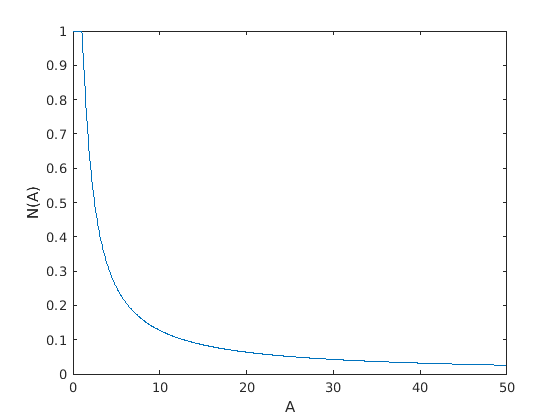
\includegraphics[width=0.6\textwidth]{figures/lab4_1_d_ganho_saturacao.png}
    \caption{Ganho aproximado da saturação em função da amplitude da frequência de entrada.}
    \label{fig:figures-lab4_ganho_saturacao-png}
\end{figure}

Analisou-se, então, a estabilidade do sistema de maneira similar, utilizando o ganho $K'$ da mesma forma que feito previamente. Como sabemos, $0 < K' < 30$. Temos que $0 < N(A) \le 1 \forall A>0$, portanto, como $K=20$, garantimos que o ganho $K'$ respeitará as condições de estabilidade com folga em relação à margem superior, mas se aproximando da instabilidade conforme $A\to \infty$ [REVISAR]. Assim, espera-se que o sistema não possua nenhum ciclo limite.

Ainda mais, pode-se esperar que o sistema se comporte bastante próximo à um sistema linear quando o ponto de referência se encontrar na região linear da saturação. Entretanto, o sistema será incapaz de atingir valores de referência superiores àqueles referentes às extremidades da saturação.

Os resultados da simulação podem ser vistos na figura \ref{fig:figures-lab4_1_d}.

\begin{figure}[H]
    \centering
    \begin{subfigure}{0.45\textwidth}
	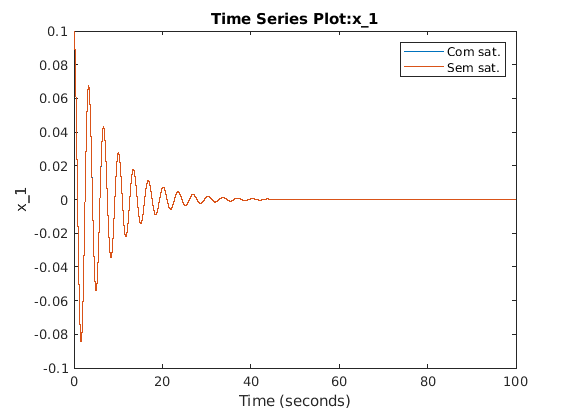
\includegraphics[width=\textwidth]{figures/lab4_1_d_sat_y_r_0.png}
	\caption{$x_{1_0}=1$ e $y_r=0$.}
    \end{subfigure}
    \begin{subfigure}{0.45\textwidth}
	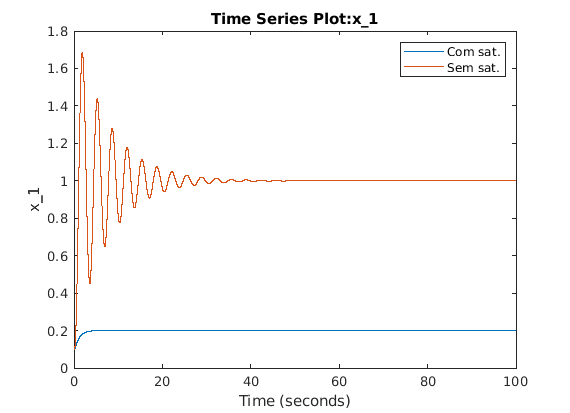
\includegraphics[width=\textwidth]{figures/lab4_1_d_sat_y_r_1.png}
	\caption{$x_{1_0}=1$ e $y_r=1$.}
    \end{subfigure}
    \caption{Resposta do sistema com e sem saturação.}
    \label{fig:figures-lab4_1_d}
\end{figure}

Em relação aos pontos de equilíbrio, tem-se a intuição de que eles encontram-se na zona linear da saturação. Verifica-se essa intuição seguindo a mesma lógica anterior. Concluímos que o equilíbrio existe para $y_r = \frac{1}{5}\phi\left( \overline{x}_3 \right) $. Como $\phi\left( \overline{x}_3 \right) \in \left[ -M,M \right]$, pode-se afirmar que o equilíbrio existe para $y_r \in \left[ -\frac{1}{5}, \frac{1}{5} \right] $. Portanto, os pontos de equilíbrio tem a forma \[
\bm{\overline{x}} = \begin{bmatrix} y_r \\ 5y_r \\ 0 \end{bmatrix} 
\] para os valores de $y_r$ que respeitem a condição definida, o que confirma a hipótese e os resultados encontrados na simulação.

\exercise{E2}

\subsubsection*{Sistema E1}

Para o sistema definido por \[
    G(s) = \frac{s+1}{s^2}
\] com ganho unitário, temos uma saturação com parâmetros $M=h=0,4$. Podemos aproximar a saturação pelo ganho \[
    N(A) = \begin{cases}
	1,& A<0,4 \\
	\frac{2}{\pi}\left( \sin^{-1}\left( \frac{0,4}{A} \right) + \frac{0,4}{A^2}\sqrt{A^2 - 0,16}  \right),& A\ge 0,4
    \end{cases}
\].

Analisamos a existência de ciclos limite então, através do lugar das raízes do sistema, visível na figura \ref{fig:figures-lab4_2_1_rlocus-png}.

\begin{figure}[H]
    \centering
    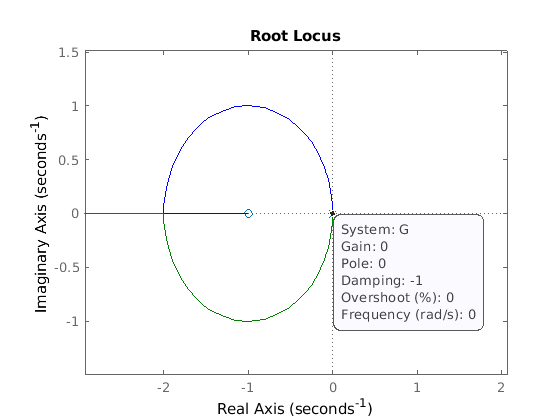
\includegraphics[width=0.8\textwidth]{figures/lab4_2_1_rlocus.png}
    \caption{Lugar das raízes do primeiro sistema.}
    \label{fig:figures-lab4_2_1_rlocus-png}
\end{figure}

Vê-se que o sistema é estável para quaisquer valores de ganho, ou seja, pela aproximação do sistema, como o ganho equivalente $K' = KN(A)$ é sempre positivo, o sistema é sempre estável e não apresenta ciclo limite.

\subsubsection*{Sistema E2}

Para o sistema definido por \[
    G(s) = \frac{(s+1)^{2}}{s^{3}}
\] com ganho $K=2$ e saturação parametrizada por $M=h=1$, pode-se aproximar a não-linearidade pelo ganho \[
    N(A) = \begin{cases}
	1,& A<1 \\
	\frac{2}{\pi}\left( \sin^{-1}\left( \frac{1}{A} \right) + \frac{1}{A^2}\sqrt{A^2 - 1}  \right),& A\ge 1
    \end{cases}
\], tal qual no item d) do primeiro exercício.

Analisou-se a existência de ciclos limite, então, pelo lugar das raízes do sistema. Conforme já analisado no relatório anterior, o sistema é instável para ganho equivalente $K' < 0,5$, portanto, para o ganho fornecido, isso implica
\begin{align*}
    &N(A) < 0,25 \\
    &\implies A > 5,06
\end{align*}
aproximadamente. Ou seja, para sinais de erro com amplitude maior que $2,53$, o sistema ficará instável.

\subsubsection*{Sistema E3}

Para o sistema definido por \[
    G(s) = \frac{1}{s(s^2+0.2s+1)}
\], com ganho $K=0,5$ e saturação com parâmetros $M=h=0,1$, pode-se aproximar a saturação por um ganho \[
    N(A) = \begin{cases}
	1,& A<0,1 \\
	\frac{2}{\pi}\left( \sin^{-1}\left( \frac{0,1}{A} \right) + \frac{0,1}{A^2}\sqrt{A^2 - 0,01}  \right),& A\ge 0,1
    \end{cases}
\].

A estabilidade do sistema foi analisada através do lugar das raízes do sistema, que indica um sistema estável para ganho equivalente $K'<0,2$. Portanto, tem-se
\begin{align*}
    &N(A) < 0,4 \\
    &\implies A > 6,28
\end{align*}
aproximadamente. Assim, temos que o sistema entra em um ciclo limite estável.

\end{document}
